\chapter{Functional Decomposition and Solutions}
\label{sec:functional_decomposition_solution}
\section{Session Overview}

Functional decomposition helps your group move from customer needs and specifications toward actual concept generation. Instead of thinking immediately about one final design, you first break the product into functions, identify the most critical sub-functions, and search for multiple ways to solve them.

By the end of this session, you should be able to:
\begin{enumerate}
    \item choose an appropriate decomposition approach for the selected product;
    \item describe functions using generic verb--noun pairs;
    \item build a requirement--function matrix; and
    \item document multiple solution options for critical sub-functions.
\end{enumerate}

\section{What Is Functional Decomposition?}

Functional decomposition breaks a complex product into smaller functional elements so that the team can understand what the product must \emph{do} before deciding exactly how it will do it. Good functional descriptions stay general. For example, \textit{move solution} is better than \textit{use a 12 V pump}, because the first phrase keeps the design space open.

\section{Decomposition Approaches}

Choose one approach that best fits your product and explain why.

\begin{itemize}
    \item \textbf{Functional decomposition}: groups the product by what it must do, using verb--noun pairs such as \textit{store solution}, \textit{move solution}, or \textit{monitor level}.
    \item \textbf{Sequence of user actions}: follows what the user does step by step, such as \textit{fill tank}, \textit{start system}, \textit{check display}, and \textit{clean parts}.
    \item \textbf{Key customer needs}: organises the product around major needs such as easy monitoring, stable flow, or easy maintenance.
\end{itemize}

Functional decomposition is usually the strongest option when the product contains technical subsystems and the team needs to understand how the functions interact.

\section{Pre-Class Activity 1: Decompose the Product}

Before class, analyse the product individually and prepare a first draft of the functional structure.

\subsection{Procedure}

\begin{enumerate}
    \item Choose one of the following approaches for problem decomposition:
    \begin{enumerate}
        \item Functional decomposition
        \item Decomposition by sequence of user actions
        \item Decomposition by key customer needs
    \end{enumerate}
    Justify the selected approach and apply it to the chosen product.

    \item Use suitable visual representations, such as function diagrams or flowcharts, to illustrate the decomposition process and the relationships among components or subfunctions.

    \item State each functional element using a \textbf{verb--noun} structure. For example, for a nutrient delivery concept, a simple function list could include:
    \begin{itemize}
        \item Store Solution
        \item Move Solution
        \item Distribute Flow
        \item Monitor Level
        \item Simplify Cleaning
    \end{itemize}

    \item Provide a brief write-up explaining how each functional element works within the overall product system to improve clarity and understanding.

    \item At this stage, the objective is to describe the product in terms of its functional elements only, without suggesting a specific technological principle for the concept.

    \item Avoid fixing the functions to a single technical solution too early. The wording should remain sufficiently broad to allow multiple concept alternatives to be developed later.
\end{enumerate}


\subsection{Decomposition Template}

Use Table~\ref{tab:session9-decomposition-template} to record your draft.

\begin{table}[htbp]
\centering
\caption{Template for documenting a decomposition approach}
\label{tab:session9-decomposition-template}
\renewcommand{\arraystretch}{1.2}
\begin{tabularx}{\textwidth}{|>{\raggedright\arraybackslash}p{0.22\textwidth}|>{\raggedright\arraybackslash}p{0.2\textwidth}|X|}
\hline
\textbf{Item} & \textbf{Draft entry} & \textbf{Notes} \\
\hline
Overall function &  &  \\
\hline
Chosen approach &  & Why this approach fits the product \\
\hline
Major sub-function 1 &  &  \\
\hline
Major sub-function 2 &  &  \\
\hline
Major sub-function 3 &  &  \\
\hline
\end{tabularx}
\end{table}

\section{Pre-Class Activity 2: Search for Solution Options}

The objective of this activity is to walk you in executing comprehensive searches and gathering solutions for critical sub-problems related to the selected product and ultimately the finding may help you in generating concepts that ensure the product's smooth functionality.

\textbf{Procedure:}
\begin{enumerate}
    \item To conduct an external search, you may consider sources such as academic publications, industry reports, technical journals, and relevant online platforms.
    \begin{enumerate}
        \item The combination between search engine and appropriate search keywords/phrases that are specific to each sub-problem may help in pinpointing/retrieving relevant information.
    \end{enumerate}
    \item Jot down and compile at least five different solutions for each critical sub-problem obtained from the external/internal search.
    \begin{enumerate}
        \item For the benefit of other reader (your team member, and module convener), it is strongly recommended to details, such as the source, author, publication date, and a brief description of each solution.
    \end{enumerate}
\end{enumerate}

For each critical sub-function, identify at least five possible solutions from internal brainstorming or external research.

\subsection{Solution Search Criteria}

When recording solutions, consider:
\begin{itemize}
    \item feasibility;
    \item alignment with the function and customer needs;
    \item technical maturity;
    \item likely resource requirements; and
    \item source credibility.
\end{itemize}

Record your findings in the template shown in Table~\ref{tab:session9-solution-template}.

\begin{table}[htbp]
\centering
\caption{Solution search template for critical sub-functions}
\label{tab:session9-solution-template}
\renewcommand{\arraystretch}{1.2}
\begin{tabularx}{\textwidth}{|>{\raggedright\arraybackslash}p{0.18\textwidth}|>{\raggedright\arraybackslash}p{0.18\textwidth}|>{\raggedright\arraybackslash}p{0.18\textwidth}|X|>{\raggedright\arraybackslash}p{0.16\textwidth}|}
\hline
\textbf{Sub-function} & \textbf{Candidate solution} & \textbf{Source} & \textbf{Description} & \textbf{Feasibility notes} \\
\hline
 &  &  &  &  \\
\hline
 &  &  &  &  \\
\hline
 &  &  &  &  \\
\hline
\end{tabularx}
\end{table}

\section{In-Class Activity 1: Agree on the Decomposition}

In class, compare the individual decompositions and agree on one shared structure.

\begin{enumerate}
    \item compare the different approaches proposed by team members;
    \item choose the approach that best matches the product and justify the choice (e.g., functional decomposition,decomposition by sequence of user actions, or decomposition by key customer needs);
    \item refine the function list so that the wording stays technology-agnostic and come out with a flowchart figures as in Figure~ \ref{fig:planting_flowchart} or the flow as in Listing~\ref{lst:seedPlanter}; and
    \item identify which sub-functions are most critical for later concept generation.
\end{enumerate}

\begin{figure}[h!]
\centering
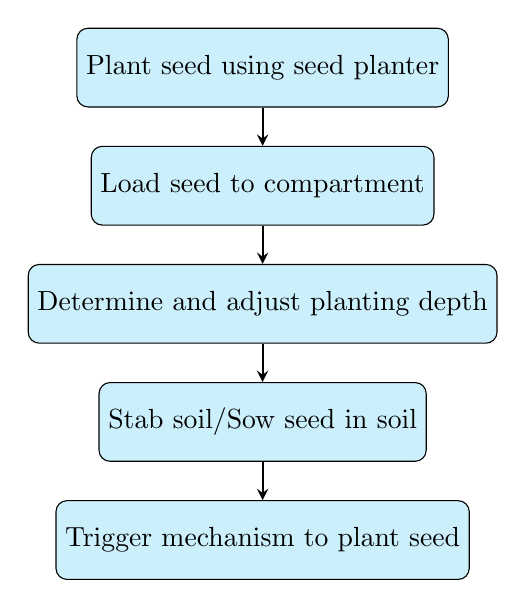
\begin{tikzpicture}[node distance=1.5cm]

\tikzstyle{startstop} = [rectangle, rounded corners, minimum width=3cm, minimum height=1cm,text centered, draw=black, fill=cyan!20]
\tikzstyle{arrow} = [thick,->,>=stealth]

\node (start) [startstop] {Plant seed using seed planter};
\node (load) [startstop, below of=start] {Load seed to compartment};
\node (depth) [startstop, below of=load] {Determine and adjust planting depth};
\node (stab) [startstop, below of=depth] {Stab soil/Sow seed in soil};
\node (trigger) [startstop, below of=stab] {Trigger mechanism to plant seed};

\draw [arrow] (start) -- (load);
\draw [arrow] (load) -- (depth);
\draw [arrow] (depth) -- (stab);
\draw [arrow] (stab) -- (trigger);

\end{tikzpicture}
\caption{Minimum planting layout in Session 8}
\label{fig:planting_flowchart}
\end{figure}

% 
\begin{center}
\begin{minted}[
  fontsize=\small,
  linenos,
  breaklines=true,
  frame=lines,
  % label=code:importJson
]{text}
Manual Seed Planter System
├── Efficient Seed Storage and Dispensing Mechanism
│   ├── Seed Metering Plate
│   ├── Seed Metering Drum
│   ├── Auger-Based Funnel
│   ├── Vibratory Feeder
│   ├── Gravity Feed Chute
│   ├── Belt Conveyor with Seed Pockets (belt with holes carrying seeds)
│   ├── Air Suction Pickup (vacuum picks and releases single seeds)
│   ├── Peristaltic Tube Dispenser (seeds squeezed along flexible tubing)
│   └── Cartridge Loading System (pre-loaded seed cartridges)
│
├── Efficient Seed Sowing
│   ├── Syringe Tip Dispensing
│   ├── Spring Loaded Gate
│   ├── Flap Valve Mechanism
│   ├── Rotating Nozzle Dispenser
│   ├── Telescopic Tube Dispenser (tube that extends downward to sow)
│   ├── Flexible Nozzle Guide (rubbery nozzle that can be aimed precisely)
│   ├── Motorized Dropper (electric controlled seed dropping)
│   └── Gravity Dropper Tube (simple tube relying on gravity but with guidance)
│
└── Planting Depth Control
    ├── Adjustable Depth Control Plate
    ├── Depth Sensor Gauge
    ├── Wheel-Based Depth Setter
    ├── Adjustable Skid Shoe
    ├── Spring-Loaded Plunger (presses the seed to a set depth)
    ├── Soil Contact Sensor (detects soil pressure to adjust depth automatically)
    ├── Telescopic Arm Adjustment (manual or motorized telescoping arm)
    └── Mechanical Stopper Rod (preset rod that limits downward travel)
\end{minted}
\captionof{listing}{Manual Seed Planter System Structure}
  \label{lst:seedPlanter}
\end{center}

\section{In-Class Activity 2: Build the Requirement--Function Matrix}

Once a comprehensive list of project functions has been identified, the next crucial step is to assess how well these functions align with customer needs. It is equally important to ensure that the number of functions is balanced — sufficient to cover all requirements without introducing unnecessary complexity.

To systematically perform this evaluation, we develop a Requirement vs Function Matrix as shown in Table \ref{tab:req_matrix_table}. This matrix provides a clear and organized method for mapping each customer requirement to the corresponding functions intended to fulfill them. It serves as a visual "roadmap," illustrating the connection between what needs to be achieved and how it will be accomplished.

\begin{table}[htbp]
    \centering
    \caption{Example requirement-function matrix for a hydroponic nutrient delivery concept}
    \label{tab:req_matrix_table}
    \renewcommand{\arraystretch}{1.2}
    \begin{tabularx}{\textwidth}{|>{\raggedright\arraybackslash}p{0.3\textwidth}|*{5}{>{\centering\arraybackslash}X|}}
        \hline
        \textbf{Requirement} & \textbf{Store solution} & \textbf{Move solution} & \textbf{Monitor level} & \textbf{Reduce leakage} & \textbf{Simplify cleaning} \\
        \hline
        Nutrient level is easy to monitor &  &  & X &  &  \\
        \hline
        Nutrient flow remains stable & X & X &  &  &  \\
        \hline
        Product is easy to clean &  &  &  &  & X \\
        \hline
        Product is safe for indoor use & X &  &  & X &  \\
        \hline
        Product is easy to install & X & X &  &  & X \\
        \hline
    \end{tabularx}
\end{table}

% \input{session9/rfm_table_landscape_hydroponic.tex}

\section{In-Class Activity 3: Consolidate the Solution Search}

Merge the best solution options into one shared team table. Record at least five solutions for each critical sub-function and note where the evidence came from. Academic papers, patents, technical datasheets, and credible industrial sources are preferable to unsupported claims.

\section{Summary and Next Steps}

At the end of this session, your group should have a shared functional decomposition, a requirement--function matrix, and a documented list of solution options for the key sub-functions. These outputs will become the raw material for concept generation in Session 10.
